\documentclass[ignorenonframetext, professionalfonts, hyperref={pdftex, unicode}]{beamer}

\usetheme{Copenhagen}
\usecolortheme{wolverine}

%Packages to be included
%\usepackage{graphicx}

\usepackage[russian]{babel}
\usepackage[utf8]{inputenc}
\usepackage[T1]{fontenc}

%%\usepackage[orientation=landscape, size=custom, width=16, height=9.75, scale=0.5]{beamerposter}

\usepackage{textcomp}

\usepackage{beamerthemesplit}

\usepackage{ulem}

\usepackage{verbatim}

\usepackage{ucs}


\usepackage{listings}
\lstloadlanguages{bash}

\lstset{escapechar=`,
	extendedchars=false,
	language=sh,
	frame=single,
	tabsize=2, 
	columns=fullflexible, 
%	basicstyle=\scriptsize,
	keywordstyle=\color{blue}, 
	commentstyle=\itshape\color{brown},
%	identifierstyle=\ttfamily, 
	stringstyle=\mdseries\color{green}, 
	showstringspaces=false, 
	numbers=left, 
	numberstyle=\tiny, 
	breaklines=true, 
	inputencoding=utf8,
	keepspaces=true,
	morekeywords={u\_short, u\_char, u\_long, in\_addr}
	}

\definecolor{darkgreen}{cmyk}{0.7, 0, 1, 0.5}

\lstdefinelanguage{diff}
{
    morekeywords={+, -},
    sensitive=false,
    morecomment=[l]{//},
    morecomment=[s]{/*}{*/},
    morecomment=[l][\color{darkgreen}]{+},
    morecomment=[l][\color{red}]{-},
    morestring=[b]",
}

\author[Epam]{{\bf Epam}\\Low Level Programming Department}

%\institution[EPAM]{EPAM}
%\logo{\includegraphics[width=1cm]{logo.png}}

\graphicspath{{../lvee2013-winter/clipart/}{../altlinux-2014/}}
\DeclareGraphicsExtensions{.pdf, .png, .jpg}


\title{Linux courses\\для разработчиков\\\href{https://github.com/epam-llpd/linux\_courses}{https://github.com/epam-llpd/linux\_courses}}

\begin{document}


\begin{frame}
	\frametitle{}
	\titlepage
	\vspace{-0.5cm}
	\begin{center}
	%\frontpagelogo
	\end{center}
\end{frame}

\begin{frame}
	\frametitle{Где взять Linux-специалистов?}

	\begin{block}{Источники}
		\begin{itemize}
			\item Система образования в РБ? \\
				LOL
			\item Существующие специалисты? \\
				Циркуляция одних и тех же лиц.
			\item Естественный приток энтузиастов? \\
				Слишком медленно.
		\end{itemize}
	\end{block}

	\begin{block}{Решение}
		\begin{itemize}
			\item Самостоятельная планомерная подготовка специалистов
			\item Создание благоприятной экосистемы для самозарождения
		\end{itemize}
	\end{block}
\end{frame}


\begin{frame}[fragile]{Заинтересованные стороны}

	  \begin{itemize}
		\item MLUG
		\item EPAM Systems
		\item SaM-Solutions
		\item Promwad
		\item БГУИР
		\item БГУ
                \item ???
	  \end{itemize}
\end{frame}

\mode<all>{\begin{frame}{Collaboration Initiative}

  \begin{center}
    Мысли глобально, действуй локально

    
\includegraphics[height=0.6\textheight]{think-globally-act-locally}

    \begin{itemize}
      \item Инициатива сотрудников снизу
      \item Работаем через нейтральную открытую площадку
    \end{itemize}

  \end{center}

\end{frame}

\begin{frame}{Конкуренция между компаниями}
      
  \center\Large\alert{Конкуренции - нет}\footnote{См кол-во проектов и падение плотности специалистов}

  \center
\includegraphics[height=0.7\textheight]{penguin}

\end{frame}


\begin{frame}[fragile]{Ранняя публикация результатов}

  \begin{center}
    \alert{Release early, release offen} 

\begin{lstlisting}
  # find linux_courses/ -name "*.tex"|wc -l
  48
\end{lstlisting}

    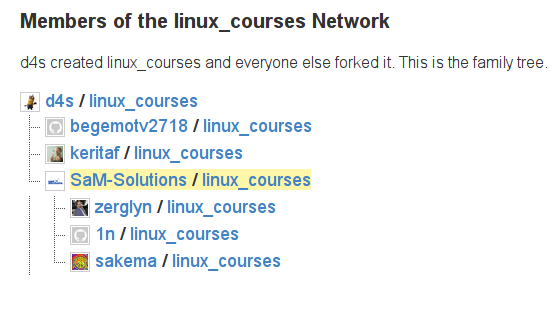
\includegraphics[width=0.65\textwidth]{members}

    \alert{Go github!}
  \end{center}
  
\end{frame}

\begin{frame}{Call for partnership}
  
  \begin{center}
    Открытый проект 'Linux образование' предлагает воспользоваться имеющимися материалами.
    
    
\includegraphics[width=0.6\textwidth]{copying}
  \end{center}

  А также с благодарностью примет:
  \begin{itemize}
    \item на хранение, распространение и доработку курсы
      \begin{itemize}
	\item незаконченные и готовые
	\item одноразовые и умершие
	\item осиротевшие
      \end{itemize}
    \item патчи
    \item баг-репорты
    \item pull-request'ы
  \end{itemize}

\end{frame}
}

\section[Epam]{Курсы Linux от Epam}

\begin{frame}{}
	\begin{columns}
		\column{0.7\textwidth}
		\Huge
		\center{Developers!\\Developers!\\Developers!\\}
		\column{0.3\textwidth}
		\center
\includegraphics[height=4cm]{steve_ballmer}
	\end{columns}
\end{frame}

\begin{frame}
	\frametitle{Курсы Linux от Epam}

	\begin{block}{Цели}
		\begin{itemize}
			\item Увеличение популярности GNU/Linux среди программистов
			\item Воспитание потенциальных сотрудников
		\end{itemize}
	\end{block}

	\begin{block}{Целевая аудитория}
		\begin{itemize}
			\item Студенты технических специальностей
			\item Программисты, желающие освоить работу в ОС Linux
		\end{itemize}
	\end{block}

	\begin{block}{Требования к кандидатам}
		\begin{itemize}
			\item Уметь программировать, под любую платформу.
		\end{itemize}
	\end{block}

\end{frame}

\begin{frame}
	\frametitle{Формат проведения занятий}

	\begin{block}{Принципы}
		\begin{itemize}
			\item Лекторы? Учителя? {\bf NO WAY!!!} \newline 
				Разработчики для разработчиков! 
			\item Небольшая группа изучающих
			\item Баланс между теорией и практикой
		\end{itemize}
	\end{block}

	\begin{block}{Место проведения}
		\begin{itemize}
			\item Совместная лаборатория Epam-БГУИР 
		\end{itemize}
	\end{block}

\end{frame}

\section[2012]{Курс 2012-2013}

\begin{frame}
  \frametitle{Первый набор (2012-2013)}
  \begin{columns}
    \column{0.5\textwidth}
	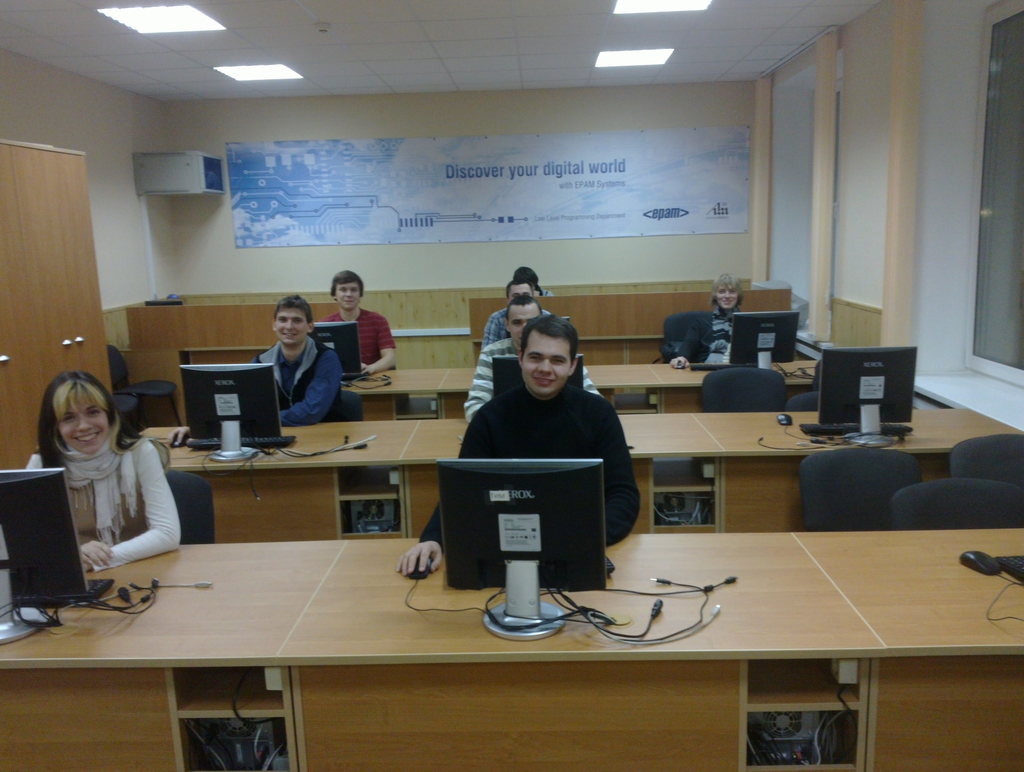
\includegraphics[width=\textwidth]{epam-evm_lab512}

    \column{0.5\textwidth}
	\begin{block}{Немного статистики}
		\begin{itemize}
			\item Подано заявок -- {\bf 39} человек
			\item После первоначального отбора: {\bf 16} человек
				\begin{itemize}
					\item из них {\bf 4} -- сотрудники Epam
				\end{itemize}
			\item Получили сертификаты -- {\bf 13} человек
			\item Устроились на Epam, как Linux-разработчики -- {\bf 4} человека
            \item Планировали 48 часов
			\begin{itemize}
    				\item[--] Получилось 66 часов
			\end{itemize}
		\end{itemize}
	\end{block}
  \end{columns}
\end{frame}

\begin{frame}
  \frametitle{Успех!}
  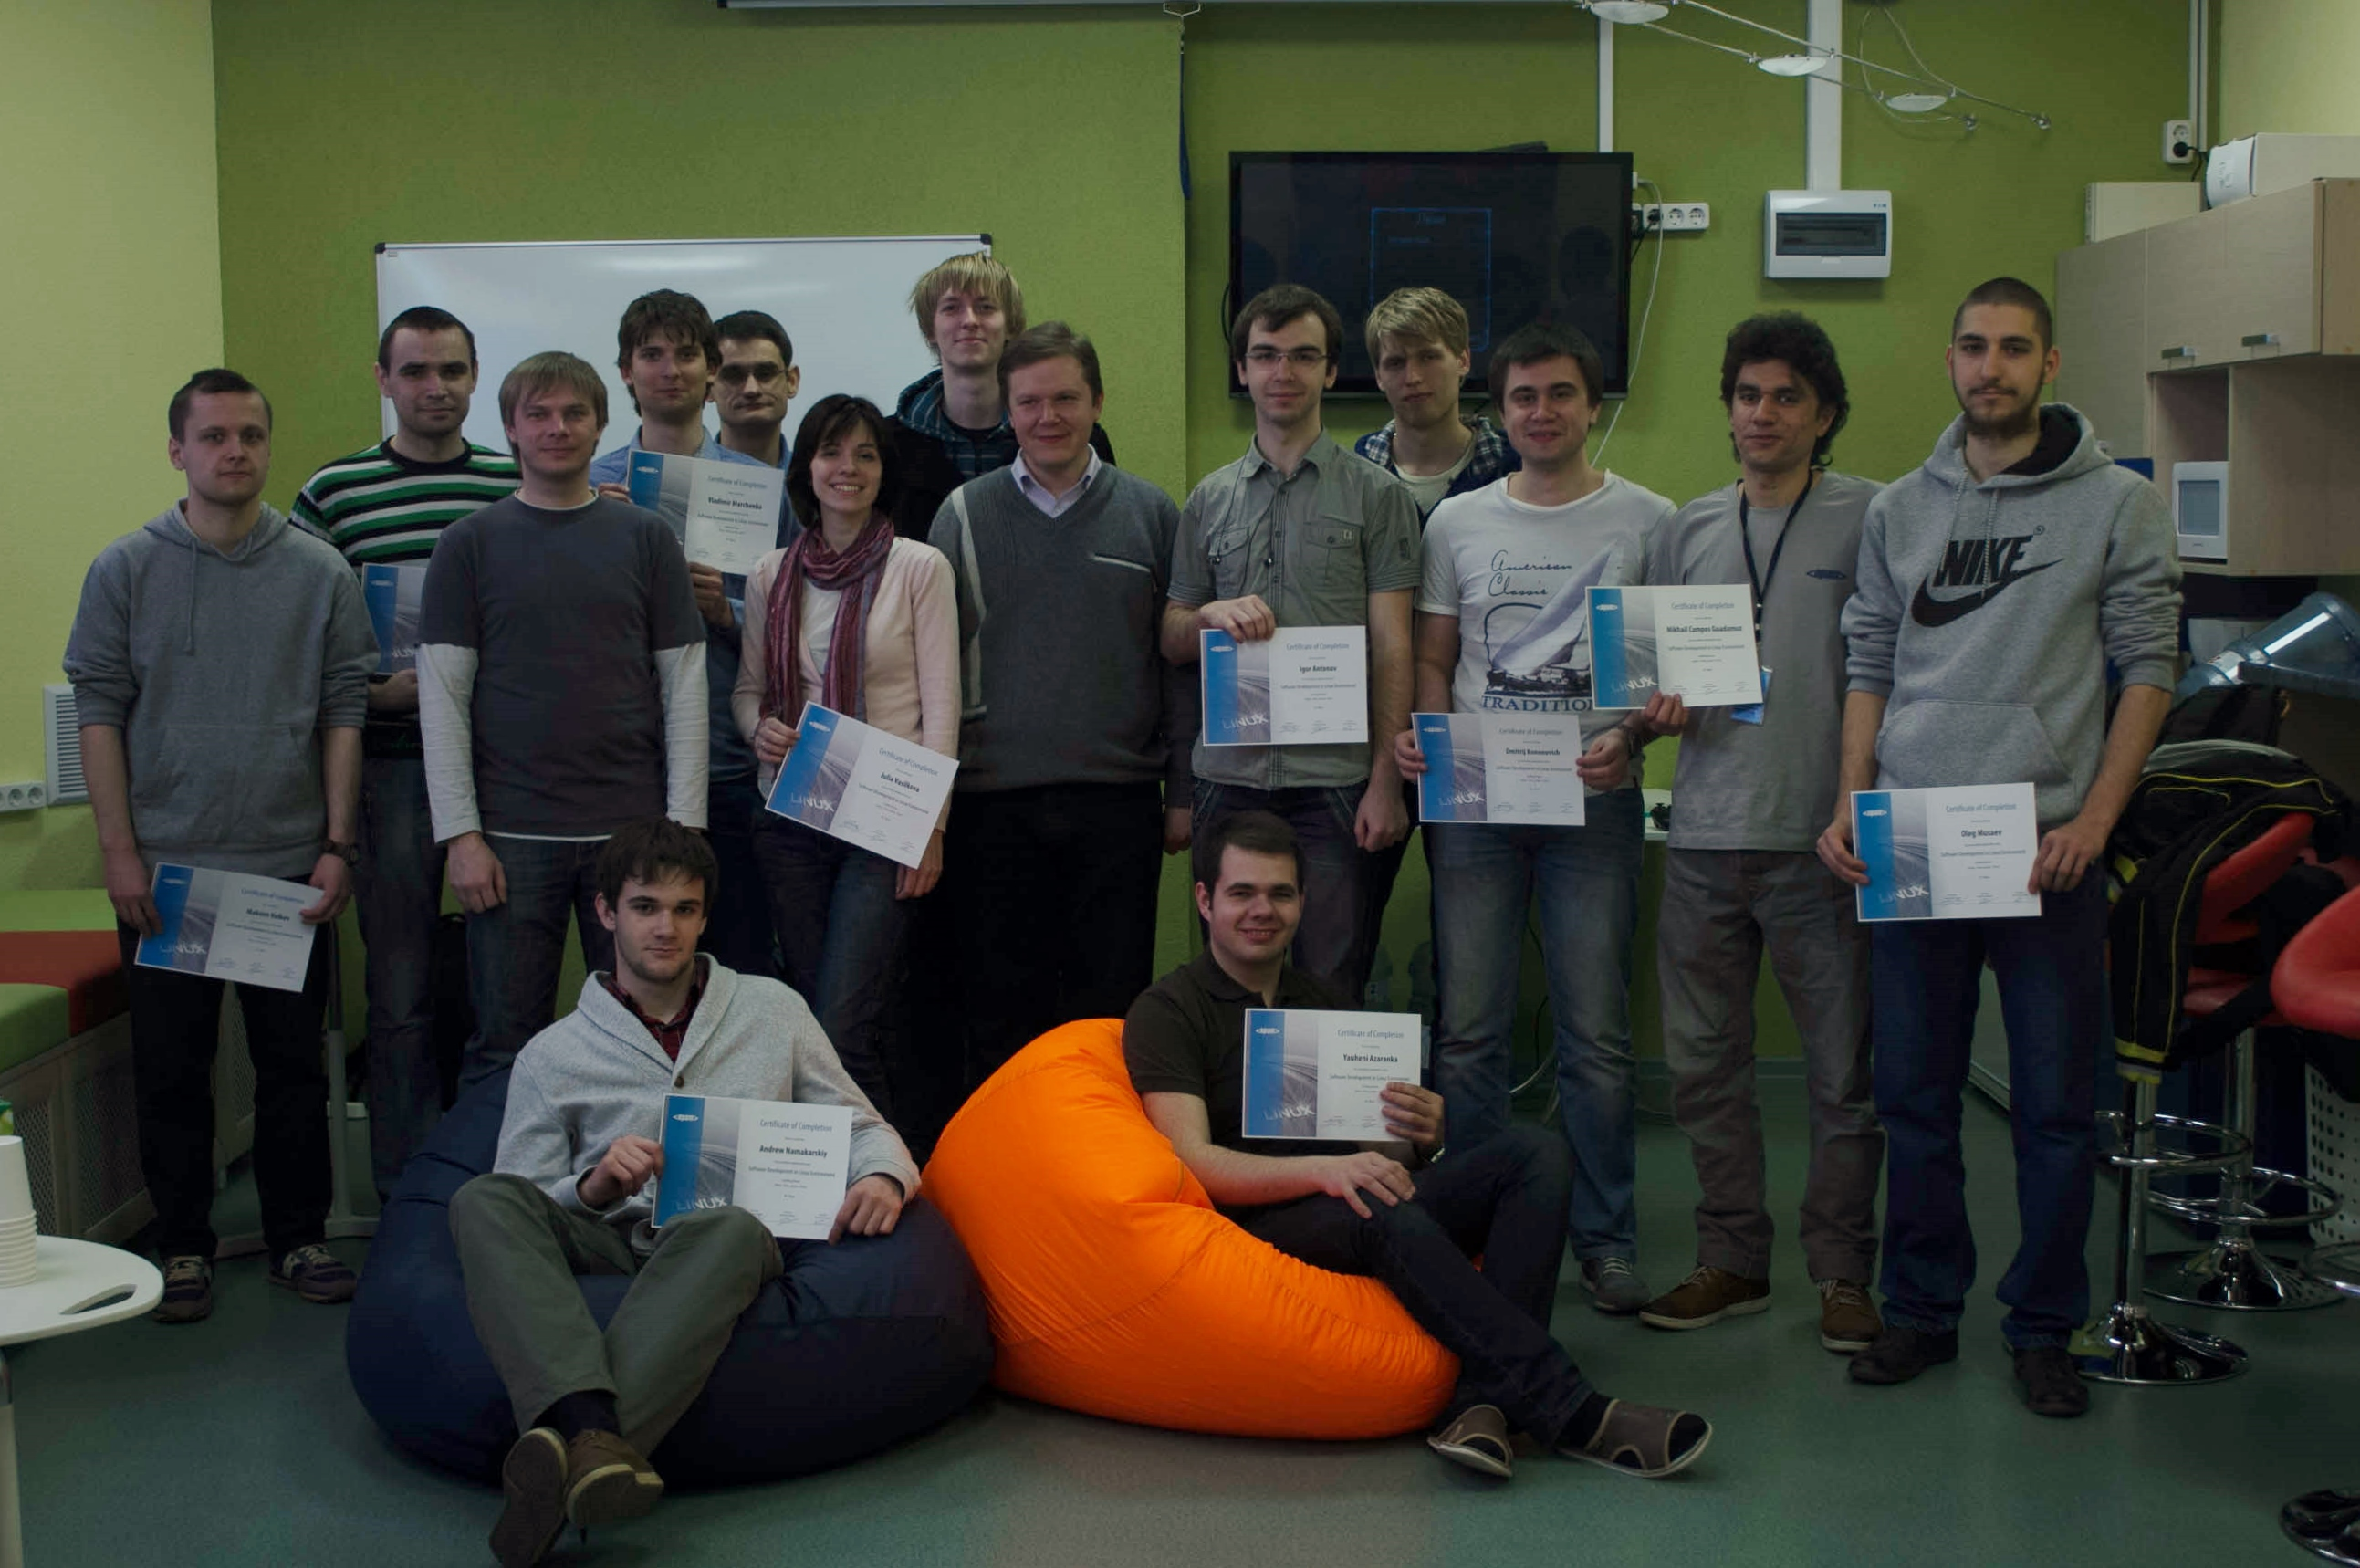
\includegraphics[width=\textwidth]{linux_courses_certificates1.jpg}
\end{frame}

\section[2013]{Курс 2013-2014}

\begin{frame}
\frametitle{Второй набор (2013-2014)}

  \begin{columns}

  \column{0.4\textwidth}

	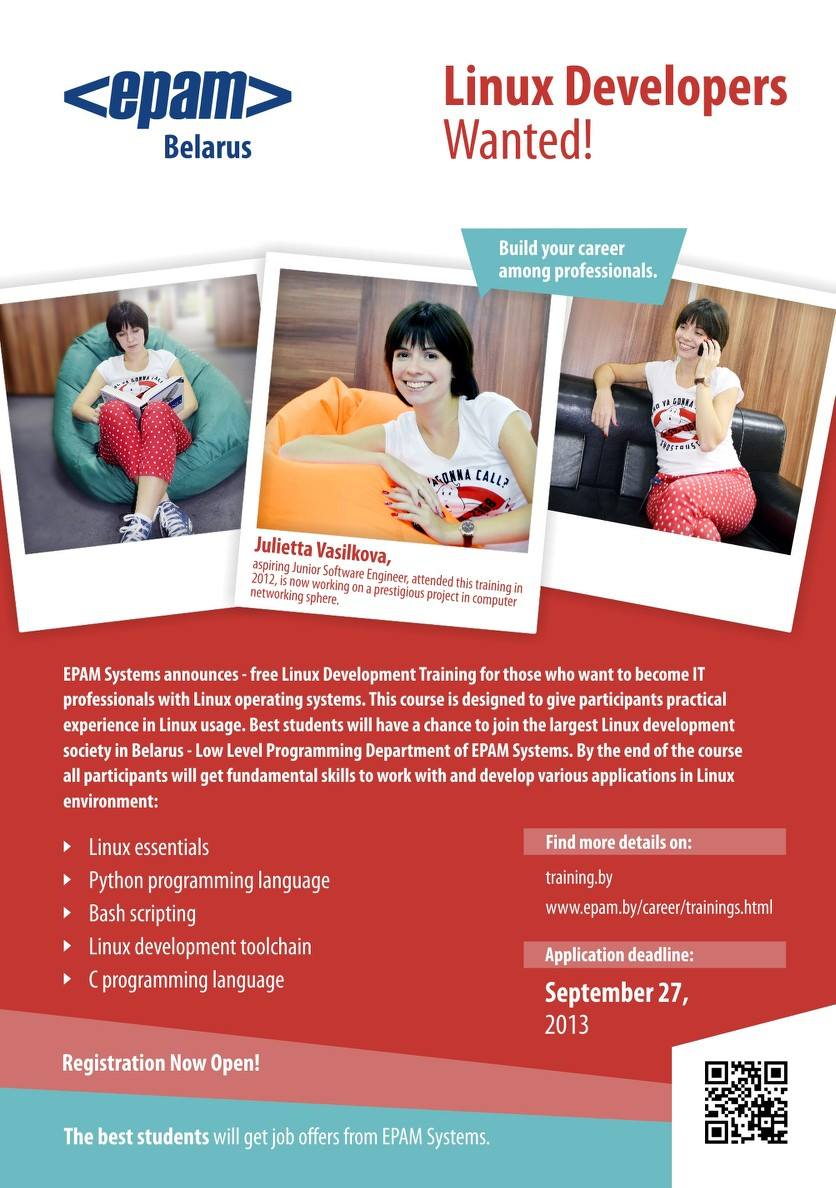
\includegraphics[width=\textwidth]{linux_courses_epam}

  \column{0.6\textwidth}
	  \begin{block}{Статистика}
		\begin{itemize}
		  \item Подано заявок: 80
		  \item Прошли телефонное интервью: 23
		  \item Дошли до курсов: 11 человек \\ + ~16 свободных слушателей (сотрудники EPAM и не только)
  		  \item Получили сертификаты -- {\bf 7} человек
		  \item Устроились на Epam, как Linux-разработчики -- {\bf 5} человека
          \item 78 (40+38) часов
		\end{itemize}
	  \end{block}
  \end{columns}
\end{frame}

\begin{frame}
\frametitle{Второй набор}
  \begin{block}{Что поменялось?}
	  \begin{itemize}
		\item Пересмотрены некоторые разделы (networking, лицензии)
		\item Добавлены новые модули
		  \begin{itemize}
	        \item Advanced C
			\item Python
		  \end{itemize}
		\item Еще два инструктора
	  \end{itemize}
  \end{block}
\end{frame}


\begin{frame}
  \frametitle{Неожиданные проблемы}

  \begin{block}{Конфликт интересов}

  \center{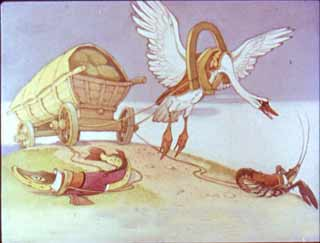
\includegraphics[width=0.3\textwidth]{Lebed_chuka_rak03.jpg}}

	\begin{columns}
		\column{0.45\textwidth}
		\begin{itemize}
			\item Введение в GNU/Linux
			\item Bash
			\item Cредства разработки, отладки и оптимизации
		\end{itemize}

		\column{0.1\textwidth}
		
		\center{\Large VS}

		\column{0.2\textwidth}
		\begin{itemize}
		  \item C
		  \item Python
		\end{itemize}
		\column{0.2\textwidth}
	\end{columns}

  \end{block}

\end{frame}

\section[2014]{Курс 2014-2015}

\begin{frame}
\frametitle{Третий набор (2014-2014)}

  \begin{columns}

  \column{0.4\textwidth}

	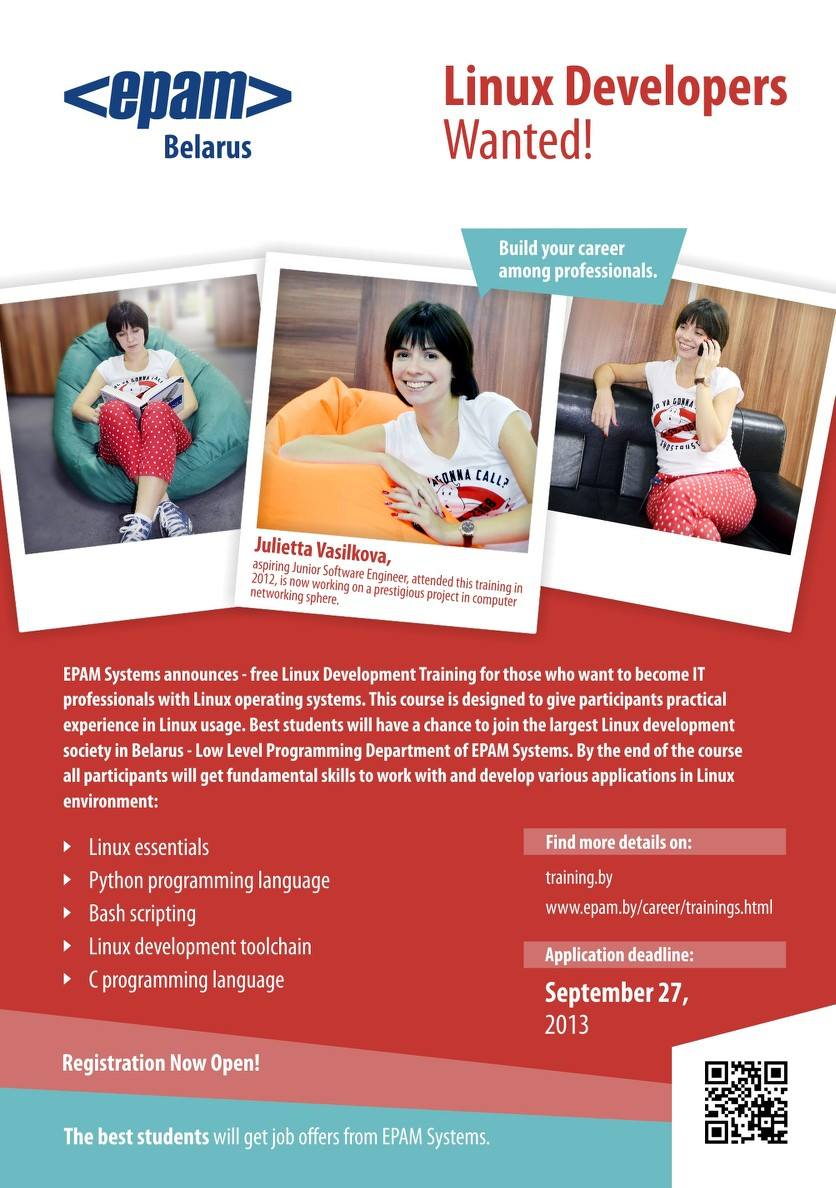
\includegraphics[width=\textwidth]{linux_courses_epam}

  \column{0.6\textwidth}
	  \begin{block}{Начало занятий}
		  Октябрь 2014
	  \end{block}
	  \begin{block}{Статистика}
		\begin{itemize}	
		  \item Подано заявок: {\bf ?}
		  \item Дошли до курсов: {\bf ?}
  		  \item Получили сертификаты: {\bf ?}
		  \item Устроились на Epam, как Linux-разработчики: {\bf ?}
          \item ~80 часов
		\end{itemize}
	  \end{block}
  \end{columns}
\end{frame}

\section{EOF}

\begin{frame}{Call for partnership}
  
  \begin{center}
    Открытый проект 'Linux образование' предлагает воспользоваться имеющимися материалами.
    
    
\includegraphics[width=0.6\textwidth]{copying}
  \end{center}

  А также с благодарностью примет:
  \begin{itemize}
    \item на хранение, распространение и доработку курсы
      \begin{itemize}
        \item незаконченные и готовые
        \item одноразовые и умершие
        \item осиротевшие
      \end{itemize}
    \item патчи
    \item баг-репорты
    \item pull-request'ы
  \end{itemize}

\end{frame}


\begin{frame}[fragile]{}

	\Large \alert{Вопросы?}\footnote{Авторы благодарят ex-сотрудника компании SaM-Solutions \\
	  Влада (mend0za) Шахова за использованные при подготовке материалы}

	\hrulefill

	\href{http://mlug.linux.by}{http://mlug.linux.by}

	\href{https://github.com/epam-llpd/linux\_courses}{https://github.com/epam-llpd/linux\_courses}

\end{frame}
\end{document}
